\section{Metode}
I dette semesterprojekt har vi arbejdet ud fra ASE-udviklingsmodellen, som er vist i figur 1. Når man arbejder ud fra denne model betyder det, at man undervejs i projektet gennemfører arbejdet i små bidder, også kaldet iterationer, og afleverer disse. I vores tilfælde har dette foregået i reviewgrupper, hvor vi har rettet hinandens dele, og herefter gennemgået rettelserne i fællesskab.
Der har været review af tre omgange; review af kravspecifikation og accepttest, review af hardware arkitektur, og slutteligt review af software arkitektur. Denne feedback har hjulpet gruppen videre ved eventuelle problemer eller tvivl.  

	\begin{figure}[h!]
	\centering
	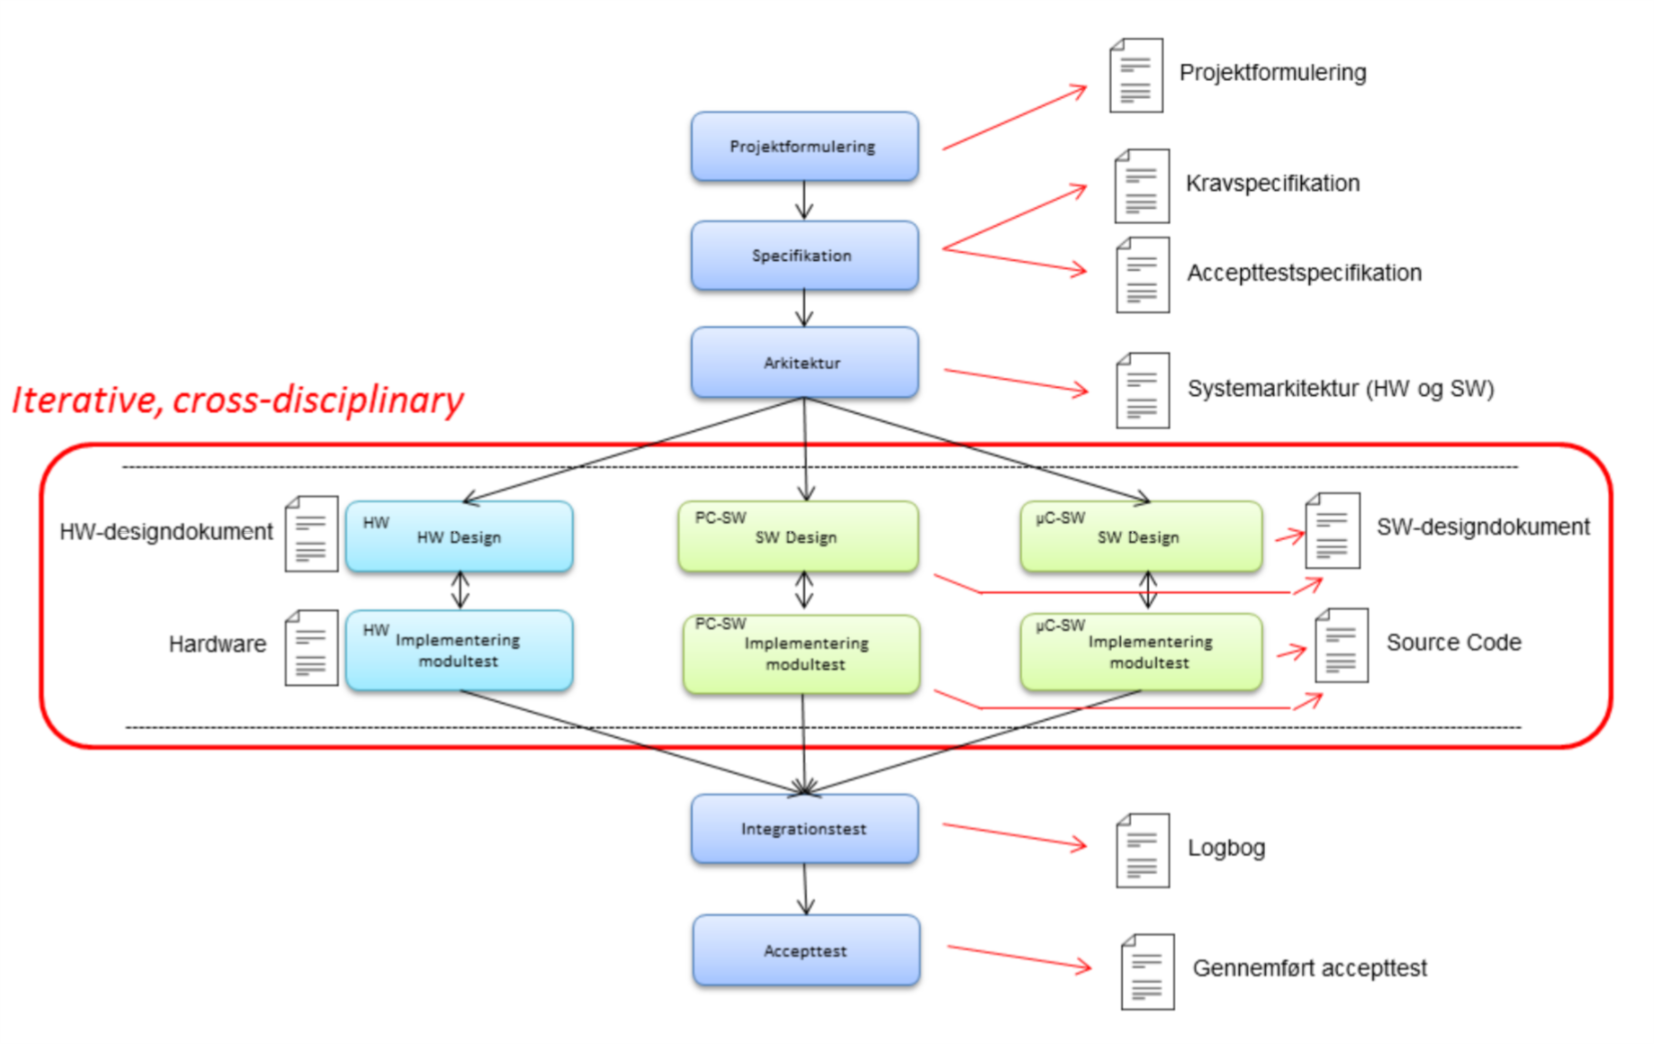
\includegraphics[width=0.8\linewidth]{Udviklingsproces/ASEmodellen}
\end{figure}

\subsection{Samarbejdsaftale}
Vi har anvendt en samarbejdsaftale, som er udarbejdet i fællesskab i gruppen[1]. Udbyttet ved brug af samarbejdsaftalen, er et bedre gruppearbejde. Når de regler og krav der er stillet til gruppemedlemmerne samt projektet, bliver formuleret og skrevet ned, vil man undgå diskussioner forvirring omkring disse, da man altid kan hive samarbejdsaftalen frem.

\subsection{Udviklingsforløb}
Som arbejdsmetoden i dette projekt, har vi anvendt Scrum. Vores projektleder Sarah har fungeret som Scrum Master, som har taget sig af det administrative og haft lederrollen. Derudover har vi benyttet os af ugentlige sprints, fra onsdag til onsdag. Til gruppemødet, som sædvanligvis ligger onsdag morgen, bliver der lavet review af det seneste sprint. Til review af sprint bliver gennemgået hvad gruppen har nået, hvilke problemer vi er stødt på, og hvordan disse er blevet løst. Herudover aftales der hvad næste uges sprint skal bestå af, og hvilke deadlines der skal være. Både review af sprint og planlægning af det nye sprint dokumenteres i et tekstdokument [2]. Udover gruppemøde ca. hver onsdag, har vi haft to ugentlige standup-møder, på omkring fem minutter. Disse møder finder sted mandag og fredag eftermiddag.
At arbejde med Scrum, som vi har gjort det, har været positivt. De ugentlige sprints har været med til at bryde projektet ned i endnu mindre dele og gøre det overskueligt. Samtidig har standup møderne giver overblik og indsigt i hvad resten af gruppen har arbejdet med og er kommet i mål med.

\subsection{Arbejdsfordeling}
Gruppen tog en beslutning om at fordele projektarbejdet i to teams; et softwareteam og et hardwareteam, da projektet er så stort at det ikke er muligt at være inde over det hele. Softwareteamet er bestående af Mathias, Nicolai og Thea, mens Hardwareteamet er bestående af Caroline, Kajene og Mikkel. Sarahs rolle er flyver, som skiftevis er med softwareteamet og hardwareteamet, alt afhængigt af hvor der er brug for ekstra hjælp.
Denne opdeling har fungeret udmærket, da den har givet mulighed for at specialisere sig, og komme dybere ned i stoffet. Dog har det også givet anledning til frustration i forhold til ikke at være helt inde over hvad det modsatte team arbejder med. De ugentlige standup-møder har bidraget til at begge teams får en forståelse for hvad der bliver arbejdet med i både hardware og software.
Projektarbejdet er også blevet uddelegeret, så hvert gruppemedlem har fået primære og sekundære områder, hvilket ses på nedenstående skema:

















